\documentclass[11pt,letterpaper]{article}
\pdfoutput=1

\usepackage{mycommands1,amssymb,amsmath,amsthm,color,pagesize,outlines,cite,subfigure,epsfig}
\usepackage[small]{caption}
\usepackage{hyperref} % for linking references
\hypersetup{colorlinks = true, citecolor = blue, urlcolor = blue}

\usepackage{stackrel}

\usepackage[round]{natbib}

% for algorithm
%\usepackage[noend]{algpseudocode}
%\usepackage{algorithm}

% DON'T change margins - should be 1 inch all around.
\addtolength{\evensidemargin}{-.5in}
\addtolength{\oddsidemargin}{-.5in}
\addtolength{\textwidth}{0.9in}
\addtolength{\textheight}{0.9in}
\addtolength{\topmargin}{-.4in}

%% measurements for 1 inch margin
%\addtolength{\oddsidemargin}{-.875in}
%\addtolength{\evensidemargin}{-.875in}
%\addtolength{\textwidth}{1.75in}
%\addtolength{\topmargin}{-.875in}
%\addtolength{\textheight}{1.75in}

%\pagestyle{myheadings}
%\markboth{}{\underline{{\bf Notes: (do not circulate)} \hspace{4.5cm} {\sc  Ansu Chatterjee} \hspace{0.25cm}}}

\DeclareMathOperator*{\ve}{vec}
\DeclareMathOperator*{\diag}{diag }
\DeclareMathOperator*{\supp}{supp }
\DeclareMathOperator*{\Tr}{Tr}
\DeclareMathOperator*{\argmin}{arg\,min}
\DeclareMathOperator*{\argmax}{arg\,max}
\DeclareMathOperator*{\Th}{^{\text{th}}}
\DeclareMathOperator*{\kl}{\text{KL}}
\DeclareMathOperator*{\rtbd}{{\colrbf tbd}}

\makeatletter
\newcommand{\opnorm}{\@ifstar\@opnorms\@opnorm}
\newcommand{\@opnorms}[1]{%
  \left|\mkern-1.5mu\left|\mkern-1.5mu\left|
   #1
  \right|\mkern-1.5mu\right|\mkern-1.5mu\right|
}
\newcommand{\@opnorm}[2][]{%
  \mathopen{#1|\mkern-1.5mu#1|\mkern-1.5mu#1|}
  #2
  \mathclose{#1|\mkern-1.5mu#1|\mkern-1.5mu#1|}
}
\makeatother

%% Appendix theorem counter
\usepackage{chngcntr}
\usepackage{apptools}
\AtAppendix{\counterwithin{Theorem}{section}}
\numberwithin{equation}{section}

\begin{document}

\newtheorem{Theorem}{Theorem}[section]
\newtheorem{Lemma}[Theorem]{Lemma}
\newtheorem{Corollary}[Theorem]{Corollary}
\newtheorem{Proposition}[Theorem]{Proposition}
\newtheorem{Conjecture}[Theorem]{Conjecture}
\theoremstyle{definition} \newtheorem{Definition}[Theorem]{Definition}
\newtheorem{Example}{Example}[section]
\newtheorem{Algorithm}{Algorithm}
\newtheorem{Remark}{Remark}

\title{Title}
\date{}
%\author{
%	Subhabrata Majumdar\thanks{Email: {\tt smajumdar@ufl.edu}}\\
%	and\\
%	George Michailidis\thanks{Corresponding author. Email: {\tt gmichail@ufl.edu}}\\
%	University of Florida, Gainesville, FL, USA
%}
\maketitle

\noindent\textbf{Abstract}: 

\vspace{.5cm}
\noindent\textbf{Keywords}:
%\newpage

\section{Formulation}
Consider a random variable $\BX \in \BR^p$ that has a sparse dependency structure among its features. This graph structure is potentially non-linear, and we want to infer the structure from a data matrix $\bfX \in \BM(n,p)$.

We assume a multi-layer generative model for the structure:
%
\begin{align*}
\bfX &= \varphi (\bfH_1) \bfB_1 + \bfE_x; \quad \BE \sim \cN_p ({\bf 0}, \Sigma_x),\\
\bfH_1 &= \varphi (\bfH_2) \bfB_2 + \bfF_1; \quad \BF_1 \sim \cN_{p_1} ({\bf 0}, \Sigma_1),\\
\cdots\\
\bfH_{L-1} &=
\varphi (\bfH_L) \bfB_L + \bfF_{L-1}; \quad \BF_{L-1} \sim \cN_{p_{L-1}} ({\bf 0}, \Sigma_{L-1}),\\
\BH_L & \sim \cN_{p_L} ({\bf 0}, \Sigma_L).
\end{align*}
%
with $L$ hidden layers, and $\varphi(\cdot)$ being a pointwise known transformation (e.g. ReLU, sigmoid, tanh).
When $\Sigma_x$ and $\Sigma_l, l \in \cI_L$ are diagonal, it is the Non-linear Gaussian Belief Network of \cite{FreyHinton99}. In our case, we keep $\Sigma_x$ non-diagonal (but sparse), while others diagonal.

The negative log-likelihood function is
%
\begin{align*}
-\ell( \bfX| \cH, \cB, \Omega) &= \frac{n}{2}\left[ \Tr \left(\bfS_x \Omega_x \right) - \log \det \Omega_x +
\sum_{l=1}^L \left\{ \Tr \left(\bfS_l \Omega_l \right) - \log \det \Omega_l \right\} \right]
\end{align*}
%
where $\bfS_x = \bfE_x^T \bfE_x/n, \bfS_l = \bfF_l^T \bfF_l/n$ for $l = 1, \ldots, L-1$ and $\bfS_L = \bfH_L^T \bfH_L/n$.
%
Inferring the distribution of the hidden variables is difficult so we assume pointwise variational approximations:
%
$$ h_{ij,l} \sim N(\mu_{ijl}, s_{ijl}); \quad i \in \cI_n, j \in \cI_{p_l}, l \in \cI_L. $$
%
Collect the variational parameters in $\cM := \{ \bfM_1, \ldots, \bfM_L\}, \cS:= \{ \bfS_1, \ldots, \bfS_L\}$. Now we have the variational lower-bound
%
\begin{align}\label{eqn:elbo}
\ell( \bfX| \cH, \cB, \Omega) \geq
\BE_q \ell (\bfX,\cH| \cB,\Omega,\cM,\cS) - \BE_q \log q(\cH| \bfX, \cB,\Omega,\cM,\cS)
\end{align}
%
Denote this lower bound by $\ell_q(\bfX|\cB,\Omega,\cM,\cS)$. Under the simplified model $\Sigma_l = \bfsigma_l \bfI$ for $l \in \cI_L$, the second term becomes \citep{FreyHinton99}
%
\begin{align}\label{eqn:KLdivergence}
\BE_q \log q(\cH| \bfX, \cB,\Omega,\cM,\cS) = \frac{1}{2} \left[\sum_{i=1}^n \sum_{j=1}^{p_l} \sum_{l=1}^L \log \frac{s_{ijl}}{\sigma_{jl}} -\frac{s_{ijl}}{\sigma_{jl}} + n \log \det \Omega_x + \text{constant} \right].
\end{align}
%
For the first term we have
%
\begin{align*}
\BE_q \ell (\bfX,\cH| \cB,\Omega,\cM,\cS) &=
\frac{n}{2} \BE_q \left[ \Tr ( \bfS_x \Omega_x) + \sum_{l=1}^L \Tr(\bfS_l \Omega_l) \right]\\
&= 
\end{align*}
%
which simplifies to \citep{FreyHinton99}
%
\begin{align}\label{eqn:loglik}
- \left[ \BE_q \Tr(\bfE_x^T \bfE_x \Omega_x)  +
\sum_{i=1}^n \sum_{j=1}^{p_l} \sum_{l=1}^{L-1}
\frac{1}{\sigma_{jl}} \left\{ (\mu_{ijl} - b_{ij,l+1} m_{ij,l+1})^2 + b_{ij,l+1}^2 v_{ij,l+1} \right\} + \text{const} \right]
\end{align}
% last layer expectation is constant
%
where $m_{ijl} = \BE_q \varphi( h_{ijl}), v_{ijl} = \BE_q (\varphi( h_{ijl}) - m_{ijl})^2$.

\subsection{Objective function}
We shall solve a penalized version of the variational lower bound in \eqref{eqn:elbo}:
%
\begin{align*}
-\frac{2}{n} \ell_q(\bfX|\cB,\Omega,\cM,\cS) + \sum_{l=1}^L \| \bfB_l\|_1 + \| \Omega_x \|_{1,\text{off}} +
P(\cM) + Q(\cS)
\end{align*}
%
with $P,Q$ being penalties over the variational parameters. We solve this using a variational (monte-carlo?) EM algorithm-

\noindent{\bf E -step}: Given values of $\cB,\Omega_x,\bfsigma_l$, solve for the variational parameters by solving
%
$$
-\frac{2}{n} \ell_q(\bfX|\cB,\Omega,\cM,\cS) + P(\cM) + Q(\cS)
$$

\noindent{\bf M -step}: Given the variational parameters, solve for the model parameters by solving an $\ell_1$-penalized version of \eqref{eqn:loglik}.

We take the greedy strategy of solving two-layer problems successively. This means molte-carlo {\it sequential} EM: first solve for the variational parameters $(\bfM_1, \bfS_1) = ((\mu_{ij,1}, s_{ij,1}))$, in the E step, then solve for $(\bfB_1,\Omega_x)$ in the M step, and continue until convergence. After that only go to the next layer. Similar to \cite{Hinton06, Bengio07}. We assume a rank-1 representation for $\bfM \equiv \bfM_1$ and $\bfS \equiv \bfS_1$:
\begin{align*}
\bfM &= \bfa \bfb^T, \bfa \in \BR^n, \bfb \in \BR^q, q \equiv p_1,\\
\bfS &= \bfc \bfd^T, \bfc \in \BR^n, \bfd \in \BR^q
\end{align*}
%
We further assume generative parameters for $\bfa$: $a_i \sim N(\mu,\sigma^2)$ for $i \in \cI_n$.

Can calculate gradients of E-step using chain rule and Appendix A of \cite{FreyHinton99}.

\begin{figure}[t]
\centering
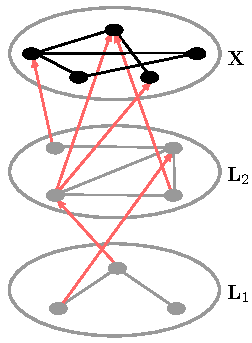
\includegraphics[height=.2\textheight]{latentmultilayer}
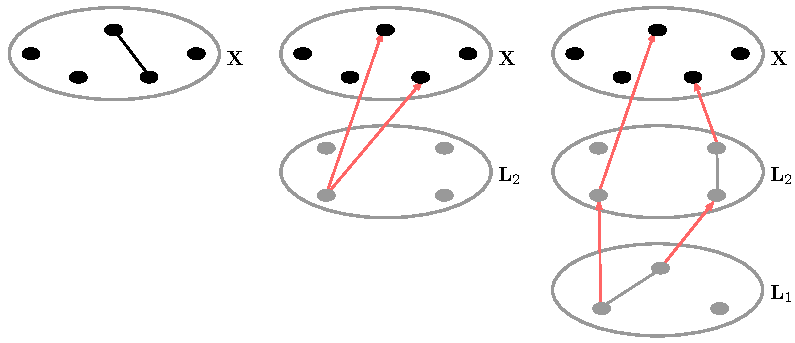
\includegraphics[height=.2\textheight]{latentinteractions}
\end{figure}

Now the objective function for a two-layer model becomes:
%
\begin{align*}
&\Tr \left[ \frac{1}{n} (\bfX - \varphi(\bfH) \bfB )^T (\bfX - \varphi(\bfH) \bfB ) \Omega_x \right] + 
\log \det \Omega_x + \| \bfB\|_1\\
\end{align*}
%

We assume the following hierarchical structures for the hidden variables and associated variational parameters:
%
\begin{align*}
h_{ij} & \sim N(\mu_{ij}, \sigma_{ij}^2),\\
\mu_{ij} & \sim \sum_{k=1}^K I_{mk} N(\mu_{mk}, \sigma_{mk}^2); \quad I_{mk} = \text{Ber}(\pi_{mk}),\\
\sigma_{ij} & \sim \sum_{k=1}^K I_{sk} N(\mu_{sk}, \sigma_{sk}^2); \quad I_{sk} = \text{Ber}(\pi_{sk}),
\end{align*}
%
Thus in total there are $6K$ variational parameters.

\paragraph{E-step:} we solve for the variational parameters by minimizing the following (take $\bfH_\varphi \equiv \varphi(\bfH)$)
%
\begin{align*}
\cF(\bfM, \bfS) &= \BE_q \Tr \left[ \frac{1}{n} (\bfX - \bfH_\varphi \bfB )^T (\bfX - \bfH_\varphi \bfB ) \Omega_x \right]\\
&= \Tr \left[ \left\{ \frac{1}{n} (\bfX - \bfM_\varphi \bfB )^T(\bfX - \bfM_\varphi \bfB ) +
\bfB^T \bfV_\varphi \bfB \right\} \Omega_x \right]\\
&= \left[ \sum_{j=1}^p \sum_{j'=1}^p \omega_{jj'} \left\{
\frac{1}{n} (\bfX_j - \bfM_\varphi \bfB_j)^T (\bfX_{j'} - \bfM_\varphi \bfB_{j'}) + \bfB_j^T \bfV_\varphi \bfB_{j'}
\right\}\right]\\
&= \sum_{j,j'=1}^p \omega_{jj'} \left\{
-\frac{2}{n} \bfX_j^T \bfM_\varphi \bfB_{j'} + \bfB_j^T \left( \frac{1}{n} \bfM_\varphi^T \bfM_\varphi + \bfV_\varphi \right) \bfB_{j'}\right\} + c
\end{align*}
%
%% variance term will be Eq ((phi(H)-M_phi)^T (phi(H)-M_phi))
where $(\bfM_\varphi)_{ik} = \BE_q \varphi (h_{ik})$ for $i \in \cI_n, k \in \cI_q$, and $\bfV_\varphi = \BE_q [(\bfH_\varphi - \bfM_\varphi)^T (\bfH_\varphi - \bfM_\varphi)/n]$. Differentiating with respect to entries of $\bfM$ we now have
%
\begin{align*}
\frac{\partial \cF}{\partial \mu_{ik}} = \sum_{j,j'=1}^p \omega_{jj'} \left[
-\frac{2}{n} x_{ij} \frac{d m_{ik}}{d \mu_{ik}} b_{j'k} +
\frac{1}{n} \left\{ 2 b_{jk} \left( 2 m_{ik} + \sum_{i' \neq i} m_{i'k} \right) \frac{dm_{ik}}{d\mu_{ik}} b_{j'k} \right\} +
{\colrbf tbd}
\right]
\end{align*}
%
Using chain rule, we get the derivatives with respect to the component vectors:
%
$$
\frac{\partial \cF}{\partial \mu} = \bfb^T \frac{\partial \cF}{\partial (\mu \bfb)}; \quad
\frac{\partial \cF}{\partial \sigma} = {\colrbf tbd}; \quad
\frac{\partial \cF}{\partial b_k} = \bfa^T \frac{\partial \cF}{\partial (b_k \bfa)}.
$$

\paragraph{M-step:} First generate data $\bfH_\varphi$ using the variational parameters $(\bfM, \bfS)$. Then obtain $\bfB,\Omega_x$ by solving a penalized LS  problem:
%
$$
\{ \hat \bfB, \hat \Omega_x \} = \argmin_{\bfB,\Omega_x} \Tr(\bfS^\varphi_x \Omega_x) + \log \det \Omega_x + \| \bfB \|_1 + \| \Omega_x \|_{\text{off},1}.
$$
%

\section{Theoretical properties}
Define equivalence classes, $\bftheta = \ve (\bfB, \Omega_{x,off})$, $\bfvt$ denoting the variational parameters, $\bfeta = (\bftheta, \bfvt)$. Then we are minimizing
%
$$
\BE_q \left[ l(\bfx; \bfz, \bfeta) + \kl(q(\bfz| \bfvt_1) \| p(\bfz)) +
\kl( r(\bfvt_1| \bfz; \bfvt) \| q(\bfvt_1; \bfvt)) \right] + P( \bftheta ).
$$
%
define the negative hierarchical ELBO by $\bar l(\cdot)$. We consider a $\ell_1$-penalty
%
$$ P(\bftheta) = \rho_1 \| \bfbeta \|_1 + \rho_2 \| \bfomega \|_1 = \lambda P_\alpha (\bftheta) $$
%
by reparameterizing the penalties: $ \lambda = \rho_1 + \rho_2, \alpha = \rho_1/\lambda$.

Conditions 1, 2, 3 same as those in SPINN paper.

Define $V_n(\bfeta) = \BE \bar l(\bfx; \bfeta) - \bar l(\bfX; \bfeta)$, $\cE(\bfeta|\bfeta_0), \bar \cE(\bfeta|\bfeta_0)$ as in \cite{StadlerEtal10}.

\begin{Theorem}\label{thm:thm1}
Define the event
%
$$
\cT = \left\{ \sup_\bfeta \frac{ |V_n(\bfeta_0^\bfeta) - V_n(\bfeta)| }{\lambda_0 \vee
(P_\alpha(\bftheta - \bftheta_0^\bfeta) + \| \bfvt - \bfvt_0^\bfeta \|_2) }
\leq T \lambda_0 \right\}
$$
%
for $T \geq 1, \lambda_0 > 0$. Then for the solution $\hat \bfeta$ defined in $\rtbd$, we have
%
$$
\cE(\hat \bfeta ) + \frac{\lambda - 2T\lambda_0}{2} \| \hat \bftheta_{S^c} \|_1 \leq
\left[ (\lambda + 2T\lambda_0) (\alpha \sqrt{s_\beta} + (1-\alpha) \sqrt{s_\omega}) C_0 \right]^2
$$

\end{Theorem}

\begin{proof}[Proof of Theorem~\ref{thm:thm1}]
Just prove an equivalent lemma of \cite{StadlerEtal10}. Details $\rtbd$.

Other details similar to Thm 1 of \cite{StadlerEtal10}.

By definition we now have that
$$
\bar l(\bfX; \hat \bfeta) + \lambda P_\alpha (\hat \bftheta) \leq
\bar l(\bfX; \bfeta_0) + \lambda P_\alpha (\bftheta_0)
$$
%
for any $\bfeta_0 \in \cQ_0$. Adding $\cE(\hat \bfeta) = \BE \bar l(\bfx; \hat \bfeta) - \BE \bar l(\bfx; \bfeta_0)$ on both sides, we get
%
\begin{align}
\cE(\hat \bfeta) + \lambda P_\alpha (\hat \bftheta) & \leq
|V_n(\bfeta_0) - V_n(\hat \bfeta)| + \lambda P_\alpha (\bftheta_0) \notag \\
& \leq T \lambda_0 \left( \lambda_0 \vee (P_\alpha (\hat \bftheta - \bftheta_0 ) +
\| \hat \bfvt - \bfvt_0 \|_2) \right) + \lambda P_\alpha (\bftheta_0) \label{eqn:thm1eqn1}
\end{align}
%
on the set $\cT$. There are three cases now.

\paragraph{Case I.} Suppose $\lambda_0 \geq P_\alpha (\hat \bftheta - \bftheta_0) + \| \hat \bfvt - \bfvt_0 \|_2$. Then rearranging the terms in \eqref{eqn:thm1eqn1} we have
%
$$
\cE(\hat \bfeta) + \lambda P_\alpha (\hat \bftheta_{S^c}) \leq
T \lambda_0^2 + \lambda P_\alpha (\hat \bftheta_S - \bftheta_{0,S} )
\leq T \lambda_0^2 + \lambda \lambda_0
$$
%
since $\lambda_0 \geq P_\alpha (\hat \bftheta_S - \bftheta_{0,S} )$.
\end{proof}

\paragraph{Case II.} Suppose $\lambda_0 < P_\alpha (\hat \bftheta - \bftheta_0) + \| \hat \bfvt - \bfvt_0 \|_2$. Then after some rearrangement we get
%
\begin{align*}
\cE(\hat \bfeta) + (\lambda - T\lambda_0) P_\alpha (\hat \bftheta_{S^c}) & \leq
T\lambda_0 \| \hat \bfvt - \bfvt_0 \|_2 + T\lambda_0 P_\alpha (\hat \bftheta_S - \bftheta_{0,S} ) +
\lambda (P_\alpha (\bftheta_{0,S}) - P_\alpha (\hat \bftheta_S))\\
& \leq T\lambda_0 \| \hat \bfvt - \bfvt_0 \|_2 + (\lambda + T \lambda_0) P_\alpha (\hat \bftheta_S - \bftheta_{0,S} )
\end{align*}

\paragraph{Condition 4.} The gradient of $\bar l(\cdot)$ with respect to the model parameters is bounded above:
%
$$
\left\| \nabla_\bfeta \bar l(\bfx; \bfeta) \right\|_\infty \leq G(\bfx)
$$
%
for some function $G: \BR^p \mapsto \BR^+$. Further, there exists $c' > 0$ such that
%
$$
| \bar l(\bfx; \bfeta) - \bar l(\bfx, \bfeta')| \BI(G(\bfx) \leq M)) \leq c'
$$
%
for any $M \geq 0$ and $\bfeta, \bfeta'$.

\begin{Theorem}\label{thm:thm2}
For the choice of $\lambda_0$:
%
$$
\lambda_0 = \rtbd,
$$
%
and any $T \geq 1$, the event $\cT$ happens with probability $\geq$
%
$$
\rtbd
$$
\end{Theorem}

\begin{proof}[Proof of Theorem~\ref{thm:thm2}]
We follow an approach similar to \cite{StadlerEtal10} and \cite{FengSimon17} to obtain probability bounds for truncated versions and tails of the quantity $|V_n(\bfeta_0^\bfeta) - V_n(\bfeta)|$ after proper scaling.

\paragraph{Part I: Bounding truncated parts.} Define the following:
%
\begin{align*}
\bar V_n(\bfeta) := \BE [\bar l(\bfx; \bfeta) \BI(G(\bfx) \leq M_n)] -
\frac{1}{n} \sum_{i=1}^n\bar l(\bfx_i; \bfeta) \BI(G(\bfx_i) \leq M_n)
\end{align*}
%
so that
\begin{align}
| \bar V_n(\bfeta) - \bar V_n(\bfeta_0) | & \leq
\BE [| \bar l(\bfx; \bfeta) -  \bar l(\bfx; \bfeta_0)| \BI(G(\bfx) \leq M_n)] + \notag\\
& \frac{1}{n} \sum_{i=1}^n | \bar l(\bfx_i; \bfeta) -  \bar l(\bfx_i; \bfeta_0)| \BI(G(\bfx_i) \leq M_n)
\label{eqn:thm2eqn1}
\end{align}
%
To get an upper bound on the right hand side of \eqref{eqn:thm2eqn1}, we start by bounding the entropy of the functional class $\cE_r, r >0$:
%
\begin{align*}
\Theta_r & := \{ \bfeta = (\bftheta, \bfvt): 
P_\alpha(\bftheta - \bftheta_0) + \| \bfvt - \bfvt_0 \|_2 \leq r \}\\
\cE_r & := \left\{ \bar l(\bfx; \bfeta) -  \bar l(\bfx; \bfeta_0) \BI(G(\bfx) \leq M_n): \bfeta \in \Theta_r
\right\}
\end{align*}
%
with respect to the empirical norm $\| h \|_{P_n} = \sqrt{\sum_{i=1}^n h^2 (\bfx_i)/n}$.

\begin{Lemma}\label{lemma:thm2lemma1}
For a collection of functions $\cH$ taking values in $\cX$, denote its metric entropy by $H(\cdot, \cH, \|.\|_{P_n})$. Then for any $u, r, M_n>0$ and some $c_0 > 0$ the following holds:
%
$$
H(u, \cE_r, \|.\|_{P_n}) \leq \frac{ (5 + c_0) r^2 M_n^2}{u^2}
\log \left(1 + \frac{d u^2}{r^2 M_n^2} \right)
$$
%
\end{Lemma}

\begin{proof}[Proof of Lemma~\ref{lemma:thm2lemma1}]
For any $\bfeta, \bfeta' \in \Theta$, due to the mean value theorem there exists $\bfeta''$ so that
%
\begin{align}\label{eqn:thm2lemma1eqn1}
\left\| \nabla_\bfeta \bar l(\bfx; \bfeta)|_{\bfeta = \bfeta''} \right\|_\infty =
\frac{| \bar l(\bfx; \bfeta) -  \bar l(\bfx; \bfeta')|}{\| \bfeta - \bfeta'\|_1}.
\end{align}
%
Define $e_\bfeta(\bfx) = | \bar l(\bfx; \bfeta) -  \bar l(\bfx; \bfeta_0)| \BI(G(\bfx) \leq M_n)$. Then, combining \eqref{eqn:thm2lemma1eqn1} with Condition (4) we get
%
\begin{align}
| e_\bfeta (\bfx) - e_{\bfeta'} (\bfx) | & \leq | \bar l(\bfx; \bfeta) -  \bar l(\bfx; \bfeta')| \BI(G(\bfx) \leq M_n) \notag\\
& \leq M_n( \| \bftheta - \bftheta'\|_1 + \| \bfvt - \bfvt' \|_1) \notag\\
& \leq M_n( \| \bftheta - \bftheta'\|_1 + \sqrt{6K} \| \bfvt - \bfvt' \|_2) \label{eqn:thm2lemma1eqn2}
\end{align}
%
so that for $u > 0$,
%
\begin{align}\label{eqn:thm2lemma1eqn3}
H(u, \cE_r, \|.\|_{P_n}) & \leq
H\left( \frac{u}{M_n}, \left\{ \bfvt: \| \bfvt - \bfvt_0 \|_2 \leq \frac{r}{\sqrt{6K}} \right\}, \|.\|_2 \right) + \notag\\
& H\left( \frac{u}{M_n}, \left\{\bftheta: \| \bftheta - \bftheta_0 \|_1 \leq r \right\} , \|.\|_2 \right) 
\end{align}
%
The first term is bounded above by $6K \log(5r M_n/(\sqrt{6K}u))$ \citep{StadlerEtal10}. Also $\log x/x \leq 1/e$ for any $x > 0$ implies that
%
$$
6K \log \left( \frac{5 r M_n}{\sqrt{6K} u} \right) = 3K \log \left( \frac{25 r^2 M_n^2}{6K u^2} \right) \leq
\frac{25 r^2 M_n^2}{2e u^2} \leq \frac{5 r^2 M_n^2}{u^2}
$$
%
For the second term, we use Lemma 2.6.11 in \cite{vdvWellnerBook96} to obtain
%
$$
H\left( \frac{u}{M_n}, \left\{\bftheta: \| \bftheta - \bftheta_0 \|_1 \leq r \right\} , \|.\|_2 \right) \leq
\frac{ c_0 r^2 M_n^2}{u^2} \log \left(1 + \frac{d u^2}{r^2 M_n^2} \right)
$$
%
for some $c_0 > 0$. Now putting everything back in \eqref{eqn:thm2lemma1eqn3} we have the needed.
\end{proof}

Leveraging the bound in Lemma~\ref{lemma:thm2lemma1}, we now prove that a symmetrized version of the truncated empirical process is small with high probability.

\begin{Lemma}\label{lemma:thm2lemma2}
Assume fixed $\bfX$, and Rademacher random variables $W_i, i \in \cI_n$ (defined as $P(W_i = 1) = P(W_i = -1) = 1/2$). Also define
%
\begin{align}\label{eqn:defineDelta}
\delta = ( 5 + c_0 )^{1/2} \left[ 1 + M_n 
\log \left( \frac{n \sqrt{c_1 K} M_n}{m_\alpha} \right) \sqrt{ \frac{ \log d}{n}} \right]
\end{align}
%
for constants $c_0, c_1 > 0$, and $m_\alpha := \alpha \vee (1-\alpha)$. Then for any $r>0, T \geq 1$ we have
%
$$
P \left( \sup_{\bfeta \in \Theta_r} \left| \frac{1}{n} \sum_{i=1}^n W_i (\bar l(\bfx_i; \bfeta) -  \bar l( \bfx_i; \bfeta_0)) \BI(G(\bfx) \leq M_n ) \right| \geq T r \delta \right) $$
$$ \leq C \exp \left[ - \frac{n T^2 \delta^2 m_\alpha^2 ( r^2 \vee 1)}{ C_1^2 K M_n^2} \right]
$$
%
for constants $C, C_1 > 0$.
\end{Lemma}

\begin{proof}[Proof of Lemma~\ref{lemma:thm2lemma2}]
Continuing from the right hand side of \eqref{eqn:thm2lemma1eqn2}, we have for any $\bfeta, \bfeta' \in \Theta_r$,
%
\begin{align*}
| \bar l(\bfx; \bfeta) -  \bar l( \bfx; \bfeta')|^2 \BI(G(\bfx) \leq M_n ) & \leq
6K M_n^2 \left( \| \bftheta - \bftheta'\|_1 + \| \bfvt - \bfvt' \|_2 \right)^2\\
& \leq \frac{6 K M_n^2}{m_\alpha^2}
\left( P_\alpha( \bftheta - \bftheta_0) + \| \bfeta - \bfeta_0 \|_2 + \right.\\
& \qquad \left. P_\alpha( \bftheta' - \bftheta_0) + \| \bfeta' - \bfeta_0 \|_2 \right)^2\\
& \leq \frac{24 K M_n^2 r^2}{m_\alpha^2}
\end{align*}
%
Now applying second part of Condition 4 we get
%
\begin{align}\label{eqn:thm2lemma2eqn1}
\frac{1}{n} \sum_{i=1}^n | \bar l(\bfx_i; \bfeta) -  \bar l( \bfx_i; \bfeta')|^2 \BI(G(\bfx) \leq M_n ) \leq
\frac{c_1 K M_n^2 ( r^2 \wedge 1)}{m_\alpha^2} := R_n^2.
\end{align}
%
Also, say $\tilde R_n^2 = c_1 K M_n^2 r^2 /m_\alpha^2$. Now using Lemma~\ref{lemma:thm2lemma1} we have
%
\begin{align}
\int_{r/n}^{R_n} H^{1/2} (u, \cE_r, \|.\|_{P_n}) du & \leq
\int_{r/n}^{\tilde R_n} H^{1/2} (u, \cE_r, \|.\|_{P_n}) du \notag\\
& \leq ( 5 + c_0 )^{1/2}  \int_{r/n}^{\tilde R_n}
\frac{ r M_n }{u} \log^{1/2} \left( 1 + \frac{ d u^2}{r^2 M_n^2} \right) du \label{eqn:thm2lemma2eqn2}
\end{align}
%
We now use the following general lemma:
%
\begin{Lemma}\label{lemma:thm2lemma3}
For any $t > 0$, we have $\log(1+t) \leq \log 2 + |\log t|$.
\end{Lemma}

\begin{proof}[Proof of Lemma~\ref{lemma:thm2lemma3}]
%The log-sum inequality \citep{LogSumBook} states that for non-negative reals $p_1, \ldots, p_m$ and $q_1, \ldots, q_m$, we have
%%
%$$
%\sum_{i=1}^m p_i \log \left( \frac{p_i}{q_i} \right) \geq \left( \sum_{i=1}^m p_i \right)
%\log \left( \frac{\sum_i p_i}{\sum_i q_i} \right).
%$$
%%
%Now take $m = 2, p_1 = q_1 = q_2 = 1, p_2 = t$. This gives
%%
%\begin{align*}
%t \log t & \geq (1+t) \log \left( \frac{1 + t}{2} \right)\\
%\Rightarrow \log(1+t) & \leq \frac{t}{1+t} \log t + \log 2 < \log t + \log 2.
%\end{align*}
If $t \geq 1$, we have $\log(1+t) \leq \log(2t) = \log 2 + \log t$. Else $\log (1+t) < \log(1 + 1/t) = \log(t+1) + |\log t| < \log 2 + |\log t|$.
\end{proof}

Thus
%
$$
\log^{1/2} \left( 1 + \frac{ d u^2}{r^2 M_n^2} \right) \leq
\sqrt{\log 2} + \sqrt{ \log d} + \sqrt{ \left| \log \left( \frac{ u^2}{r^2 M_n^2} \right) \right| }.
$$
%
Putting this back in \eqref{eqn:thm2lemma2eqn2},
%
\begin{align}
\frac{1}{\sqrt n} \int_{r/n}^{R_n} H^{1/2} (u, \cE_r, \|.\|_{P_n}) du & \leq
( 5 + c_0 )^{1/2} \left[ 1 + \sqrt{ \frac{ \log d}{n}} \int_{r/n}^{\tilde R_n} \frac{r M_n}{u} du \right] \notag\\
& = ( 5 + c_0 )^{1/2} \left[ 1 + r M_n 
\log \left( \frac{n \tilde R_n}{r} \right) \sqrt{ \frac{ \log d}{n}} \right] \notag\\
& = ( 5 + c_0 )^{1/2} \left[ 1 + r M_n 
\log \left( \frac{n \sqrt{c_1 K} M_n}{m_\alpha} \right) \sqrt{ \frac{ \log d}{n}} \right]
\label{eqn:thm2lemma2eqn3}
\end{align}
%
Take $\delta$ as in \eqref{eqn:defineDelta}. We now apply Lemma 3.2 in \cite{vandeGeerBook00} on the functional class $\cE_r$. Combining \eqref{eqn:thm2lemma2eqn1} and \eqref{eqn:thm2lemma2eqn3}, all conditions of the lemma are satisfied. Thus we obtain
%
$$
P \left( \sup_{\bfeta \in \Theta_r} \left| \frac{1}{n} \sum_{i=1}^n W_i (\bar l(\bfx_i; \bfeta) -  \bar l( \bfx_i; \bfeta_0)) \BI(G(\bfx) \leq M_n ) \right| \geq \delta \right) \leq
C \exp \left[ - \frac{n \delta^2}{ C^2 R_n^2} \right]
$$
%
by applying the lemma. Now replace $\delta$ by $Tr \delta$ and substitute for $R_n^2$ from right hand side of \eqref{eqn:thm2lemma2eqn1} to get the needed.
\end{proof}

\paragraph{Pat II: Bounding the tails.}
\end{proof}

%-----------------------------
%\hrulefill
%-----------------------------
%\section{Numerical performance}

\bibliographystyle{apalike}
\bibliography{NLGMbib}
\end{document}